% Compile twice with: pdflatex Review1_Report.tex
\documentclass{ssnreview}

\usepackage{amsmath}
\usepackage{amsfonts}
\graphicspath{{../Phase 1 Report/diagrams/}}

\projecttitle{PAYLOAD-AWARE TWO-TIER UAV ROUTE PLANNING FOR LAST-MILE DELIVERY}
\reviewnumber{REVIEW REPORT -- I}
\students{%
  Thirumurugan RA \hfill (3122235001149)\\
  Shrika SP Thota \hfill (3122235001125)\\
  Meghna Manimaran \hfill (3122235001079)}
\supervisor{Sujaudeen N, Assistant Professor}
\department{Department of Computer Science and Engineering}
\institution{Sri Sivasubramaniya Nadar College of Engineering}
\academicyear{2026--2027}
\collegelogo{ssn-logo.png}

\begin{document}
\makereviewtitle
\reviewfrontmatter

% ============================================================
\begin{reviewabstract}
UAV systems for medical and emergency last-mile delivery must balance objectives that
fundamentally conflict: shorter routes carry higher flight risk, low-risk corridors drain
more battery, and energy-efficient paths are rarely the fastest. No single fixed
trade-off serves all payload types, yet existing planners apply the same objective
weights to every mission regardless of what is being carried.

Existing multi-objective planners---including entropy-based, diversity-driven, and
crowding-distance Pareto selection methods---encode objective weights as a fixed scalar
before path search begins. Payload properties such as fragility class, temperature
sensitivity, and delivery urgency have no influence over which Pareto-optimal route is
chosen. When the payload changes, operators must re-tune weights manually and re-run the
planner---an intervention that is infeasible under field conditions.

This work proposes a \textit{Payload-Aware Two-Tier UAV Route Planning} system that
separates Pareto front construction from route selection, introducing an explicit
algebraic bridge between Tier~1 routing objectives and Tier~2 payload metadata. Tier~1
runs a multi-objective A*/Dijkstra graph-search over a delivery airspace graph sourced
from OpenStreetMap, producing a Pareto-optimal route set across distance, energy
consumption, and flight risk. Tier~2 reads four operator-assigned payload tags and
derives objective weights through a fixed formula: fragility class scales
$w_\mathrm{risk}$, delivery urgency scales $w_\mathrm{dist}$, and temperature
sensitivity scales $w_\mathrm{energy}$. These weights score every Pareto point through a
utility function; the $\arg\max$ is selected as the mission route.

The system will be evaluated on programmatically generated airspace graphs at three
scales (50, 200, and 500 nodes) against single-objective A* and MOPSO baselines, using
hypervolume, Pareto spread, and Tier~2 selection accuracy as metrics. Hardware
validation will be conducted using a Pixhawk-equipped quadcopter through ArduPilot SITL
simulation and outdoor flight tests. The principal contribution is a formula-driven
mapping from payload metadata to routing objective weights, connecting mission context
directly to Pareto point selection without expert intervention.

\keywords{UAV route planning; multi-objective optimisation; Pareto front; payload-aware
selection; algebraic bridge; last-mile delivery; ArduPilot}
\end{reviewabstract}

% ============================================================
\chapter{Introduction}

Unmanned aerial vehicles (UAVs) have emerged as a compelling platform for last-mile
delivery in scenarios where ground transportation is impractical---medical supply chains
to remote clinics, emergency drug drops during disaster response, and fragile diagnostic
sample transport where road vibration risks contamination. In each scenario the UAV must
fly a route from a dispatch hub to a delivery point across an airspace that contains
obstacles, regulated no-fly zones, and variable wind corridors. A good route balances
three conflicting physical objectives simultaneously: minimising total flight distance,
minimising battery energy expenditure, and avoiding high-risk segments.

The standard engineering response to such a conflict is to form a weighted sum of the
three objectives into a single scalar cost function and then run a conventional path
planner such as A* on it. This scalar collapses the multi-objective problem into a
single-objective one, and the operator adjusts the three weights to express the
mission's priority before each flight. The approach works for a fixed mission type, but
it fails immediately when the payload changes: emergency medicine requires a completely
different weight profile from fragile biological samples or disaster-relief bulk
supplies. Manually re-tuning and re-running the planner between missions is
operationally impractical in time-critical field conditions.

\section{Background}

Multi-objective UAV path planning has attracted sustained research attention because no
single route can simultaneously minimise distance, energy, and flight risk---these
objectives are structurally in conflict. The dominant approach in the literature is to
generate a Pareto-optimal front of non-dominated routes, each representing a different
trade-off across the objective space, and then select one route from that front as the
mission route.

The critical question that determines the practical value of any such system is:
\textit{how is the final route selected from the Pareto front?} The three most directly
relevant papers reviewed below all answer this question using \textbf{front diversity
metrics}: entropy, geometric spread, or crowding distance. These metrics select routes
that are well-distributed across the Pareto front, but they are entirely blind to the
delivery context. None of the three papers allow what the UAV is carrying to influence
which route is chosen. This is the structural research gap this project addresses.

Autonomous UAV systems for medical and emergency last-mile delivery operate under a
structural constraint that distinguishes them from general routing problems: the optimal
route trade-off is not fixed---it is a function of what is being carried. A fragile
diagnostic sample demands a low-vibration, low-turbulence corridor even at the cost of a
much longer flight time. Emergency insulin requires the shortest path regardless of risk.
Bulk disaster-relief supplies demand the most energy-efficient route to maximise delivery
range.

\section{Motivation}

The motivation for this work arises from three real operational scenarios that impose
fundamentally incompatible routing requirements:

\textbf{Fragile medical samples} (tissue biopsies, blood samples, pathology specimens)
are highly sensitive to vibration, g-forces, and thermal exposure. The dominant routing
priority is minimising flight risk---defined here as exposure to turbulent corridors,
sudden altitude changes, and wind-exposed segments. A route that adds 40\% extra
distance but halves the risk of vibration damage is operationally preferable.

\textbf{Emergency medicine} (insulin, epinephrine, antivenom) has a strict time window.
The dominant routing priority is minimising route distance to minimise transit time.
Flight risk and energy are secondary. For a payload with a 15-minute delivery window,
the shortest path wins unconditionally.

\textbf{Disaster-relief bulk supplies} (water purification tablets, bandages, ration
packs) weigh significantly more than medical payloads and are not time-critical or
fragile. The dominant routing priority is energy efficiency---minimising battery drain to
maximise the number of deliveries possible on a single charge cycle.

No existing UAV planner can switch between these three routing strategies based on a
payload tag. The proposed two-tier system accomplishes this without any expert
intervention or replanning. Payload metadata---fragility class, temperature sensitivity,
delivery urgency---has never been used as the sole input to autonomous Pareto point
selection in the UAV delivery literature, leaving a structural gap this project directly
addresses.

\section{Objectives}
\begin{enumerate}[label=\arabic*.]
  \item To formulate multi-objective UAV route planning as a structured \textbf{Pareto
  front pre-computation} problem over a delivery airspace graph, theoretically
  distinguishing the deterministic graph-search approach from stochastic
  population-based alternatives.
  \item To design a \textbf{payload metadata schema} and a principled rule-based mapping
  that translates mission context (fragility class, delivery urgency, temperature
  sensitivity) into Pareto point selection objective weights without any expert weight
  tuning.
  \item To benchmark Tier~1 route quality and Pareto front coverage against
  single-objective A* and MOPSO baselines on identical delivery scenarios, measuring
  hypervolume and Pareto spread (Inverted Generational Distance).
  \item To quantify \textbf{Tier~2 selection accuracy} by measuring alignment between
  selected route characteristics and payload tag requirements across diverse mission
  types (fragile medical sample, emergency medicine, disaster-relief supplies).
  \item To establish the system's \textbf{novelty}: payload metadata is used as the sole
  input to Pareto point selection, replacing context-blind entropy and diversity-based
  criteria with a deterministic algebraic mapping from payload description to route
  choice.
\end{enumerate}

\section{Scope}

This project covers two phases. Phase~I delivers a complete, validated software
simulation system including the multi-objective A* graph-search engine (Tier~1), the
payload-driven route selector (Tier~2), a MOPSO baseline, and a benchmarking suite
evaluated on programmatically generated airspace graphs at three scales (50, 200, and
500 nodes). Phase~II extends the validated software to physical hardware: a
Pixhawk-equipped F450 quadcopter with a Raspberry Pi~5 companion computer, validated
through ArduPilot SITL simulation and outdoor flight tests. The project does not address
multi-UAV coordination, dynamic obstacle avoidance during flight, or real-time path
replanning.

% ============================================================
\chapter{Related Work}

Multi-objective UAV path planning literature consistently uses Pareto front diversity
metrics---entropy, geometric spread, or crowding distance---for route selection, with no
regard for the delivery context. Three papers that are most directly relevant to the
proposed work are reviewed below. Table~\ref{tab:related-work} provides a structured
comparison.

\begin{table}[H]
\centering\caption{Summary of related work}\label{tab:related-work}\small
\begin{tabularx}{\textwidth}{>{\centering\arraybackslash}p{1.1cm} L{2.9cm} Y Y Y}
\toprule
\textbf{S.No.} & \textbf{Author/Year} & \textbf{Proposed Method} & \textbf{Key Findings} & \textbf{Limitations}\\
\midrule
1 & Chokkalingam \& Ganesan (2026) \cite{r1} &
Multi-objective UAV path planning with adaptive constraint handling and entropy-based
criterion for Pareto front selection. &
Strong Pareto front coverage versus MOPSO; entropy criterion selects routes spanning a
wider range of objective combinations than random selection. &
Payload metadata never incorporated; fragile samples and emergency medicine receive
identical route selection from the same front.\\[4pt]
2 & Datsko et al.\ (2024) \cite{r2} &
Diversity-driven Pareto selection for UAV routing that maximises geometric spread of
candidate solutions across the multi-objective space. &
Improvements in Inverted Generational Distance (IGD) over diversity-agnostic selection;
better coverage of the true Pareto front. &
Selection is guided entirely by solution diversity; delivery context, payload type, and
time window have no influence on which route is chosen.\\[4pt]
3 & Ntakolia et al.\ (2023) \cite{r3} &
Crowding-distance-based Pareto point selection in a multi-objective UAV path planner
(NSGA-II style). &
Well-spread Pareto fronts for UAV routing; compares favourably against NSGA-II and
$\varepsilon$-constraint methods on grid-world airspace environments. &
Crowding distance cannot encode urgency, fragility, or thermal sensitivity; mission
context is absent from selection at any stage.\\
\bottomrule
\end{tabularx}
\end{table}

\section{Research Gap}

All three reviewed papers select Pareto-optimal routes based on \textbf{front diversity
metrics}---entropy, geometric spread, and crowding distance respectively. None of them
allow the delivery context (what payload is being carried) to influence which route is
selected. This is the structural gap the proposed system directly addresses.

The gap is not a minor implementation detail---it is a fundamental design assumption.
Entropy, geometric spread, and crowding distance are all defined over the Pareto front
itself. They have no interface through which external mission context can enter.
Extending these methods to incorporate payload information would require replacing the
selection criterion entirely, which is precisely what the proposed Tier~2 utility
scoring mechanism does.

Three specific gaps addressed by this work are as follows. \textbf{Gap~1 (No
payload-aware Pareto selection):} All existing UAV multi-objective planners apply a
fixed selection criterion independent of payload type. The proposed Tier~2 introduces a
formula-driven mapping from four payload tags directly to Pareto point selection.
\textbf{Gap~2 (No re-use across mission types):} Existing planners re-run the full
multi-objective search when the mission context changes. The proposed two-tier separation
pre-computes the Pareto front once (Tier~1) and allows instantaneous route selection for
any new payload tag (Tier~2), without re-running the planner. \textbf{Gap~3 (No
algebraic bridge between delivery context and routing objectives):} The mapping between
a payload description and the routing trade-off it implies (e.g., fragility
$\rightarrow$ minimise risk, urgency $\rightarrow$ minimise distance) has never been
formalised algebraically. The proposed weight-derivation formula provides this bridge,
making the mapping deterministic, transparent, and reproducible.

% ============================================================
\chapter{Problem Statement}

Existing UAV route planners encode distance, energy consumption, and flight risk into a
\textbf{single hand-tuned weighted-sum scalar} before path search begins, permanently
fixing the objective trade-off regardless of what is being carried. When the payload
context changes---from fragile diagnostic samples requiring vibration-minimal routing to
time-critical emergency medicine requiring shortest-path routing---an expert must
manually re-tune the planner weights and re-run the search from scratch. This
intervention is \textbf{infeasible in field conditions}.

Formally, given:
(i)~an airspace graph $G = (V, E)$ with three-objective edge cost vectors
$\mathbf{c}(e) = [d(e),\, \varepsilon(e),\, \rho(e)]$ representing geodesic distance,
estimated energy consumption, and flight risk respectively;
(ii)~a Pareto-optimal front $\mathcal{P}$ of non-dominated routes pre-computed over $G$;
and (iii)~a payload metadata tuple $(F, T, U, P_\mathrm{lvl})$ encoding fragility class
$F \in \{1\ldots5\}$, temperature sensitivity $T \in \{1\ldots3\}$, delivery urgency
$U \in \{1\ldots3\}$, and priority level $P_\mathrm{lvl} \in \{1\ldots5\}$---the
problem is to select the route $p^* \in \mathcal{P}$ that best satisfies the routing
requirements implied by the payload metadata, without expert re-tuning and without
re-running the multi-objective search.

The inputs are measurable quantities the operator can assign from domain knowledge (e.g.,
``this vial is fragile: $F = 5$; delivery is non-urgent: $U = 1$''). The constraints are
that selection must be deterministic, reproducible, and complete within one second of
payload tag entry. The success criterion is that the selected route characteristics
(distance, energy, risk) align with the payload's stated requirements as verified by a
Tier~2 selection accuracy metric evaluated across multiple payload presets.

% ============================================================
\chapter{Justification for the Problem Formulation}

\section{Need for the Proposed Work}

No current UAV route planner adjusts its routing priorities to match the payload being
carried. The same fixed objective weights are applied to every mission, forcing field
operators to manually recalibrate between every deployment. This is impractical and
error-prone in time-critical emergency scenarios. Payload metadata (fragility class,
temperature sensitivity, delivery urgency) has never been used as the sole input to
autonomous Pareto point selection in the UAV delivery literature, leaving a structural
gap this project directly addresses.

The proposed system resolves this by separating Pareto front generation from
mission-context-driven route selection. The Pareto front is computed once for a delivery
region and stored. For each new mission, only Tier~2 runs---reading the payload tag and
selecting the appropriate route from the pre-computed front in near-instantaneous time,
with no re-planning and no expert weight adjustment required.

\section{Feasibility}

\textbf{Technical feasibility:} The Tier~1 multi-objective A*/Dijkstra algorithm is a
well-studied graph-search extension. The Tier~2 utility scoring is a closed-form
algebraic formula executable in microseconds on any hardware. Both components are
implementable in Python with standard open-source libraries (NetworkX, NumPy). Hardware
deployment on a Raspberry Pi~5 companion computer is feasible given the computational
simplicity of Tier~2 route selection ($< 1\,\mathrm{s}$ end-to-end from payload tag
input to mission file output).

\textbf{Operational feasibility:} The system requires only four integer tag inputs from
the operator, eliminating the need for weight-tuning expertise. The ArduPilot
SITL simulation environment allows complete end-to-end validation before outdoor
flights, reducing hardware risk to an acceptable level.

\textbf{Economic feasibility:} All software components use open-source libraries
(osmnx, NetworkX, NumPy, matplotlib). The hardware platform---F450 quadcopter frame,
Pixhawk flight controller, Raspberry Pi~5---uses standard, commercially available
components at modest cost. No specialised or proprietary software licences are required.

\textbf{Schedule feasibility:} Phase~I (software simulation and benchmarking) is
achievable within the first semester aligned to Review~I. Phase~II (hardware integration
and outdoor testing) is planned for the second semester, with milestones aligned to the
Review~II and Final Review schedule as shown in Chapter~\ref{cha:timeline}.

\section{Expected Contribution}

The principal contribution is a formula-driven mapping from payload metadata to routing
objective weights, connecting mission context directly to Pareto point selection without
expert intervention. This replaces context-blind diversity criteria with a direct
algebraic link from payload description to route choice. The Pareto front is computed
once and reused across all mission types without re-running the planner, making the
system both operationally efficient and reproducible. The proposed system is the first in
the UAV delivery literature to use payload metadata as the \textit{sole} autonomous input
to Pareto point selection, constituting a novel algebraic bridge between delivery context
and routing objectives.

% ============================================================
\chapter{Methodology}

The proposed system is built on a single architectural decision: \textbf{separate Pareto
front construction (Tier~1) from route selection (Tier~2)}. This separation eliminates
the need to re-run a multi-objective search each time the payload changes. The Pareto
front is computed once for a delivery region and stored persistently. For each new
mission, only Tier~2 runs---reading the payload tag and selecting the appropriate route
from the pre-computed front in near-instantaneous time.

\section{Architectural Design for Proposed System}

Figure~\ref{fig:architecture} shows the complete two-tier system architecture. Airspace
graph data from OpenStreetMap enters Tier~1, which performs a multi-objective
A*/Dijkstra search and stores the resulting Pareto-optimal route set. For each new
mission, Tier~2 reads the four operator-assigned payload tags, derives objective weights
algebraically, scores every stored Pareto point via a utility function, and outputs the
$\arg\max$ as the selected mission route along with an ArduPilot-compatible
\texttt{.waypoints} file.

\begin{figure}[H]
\centering
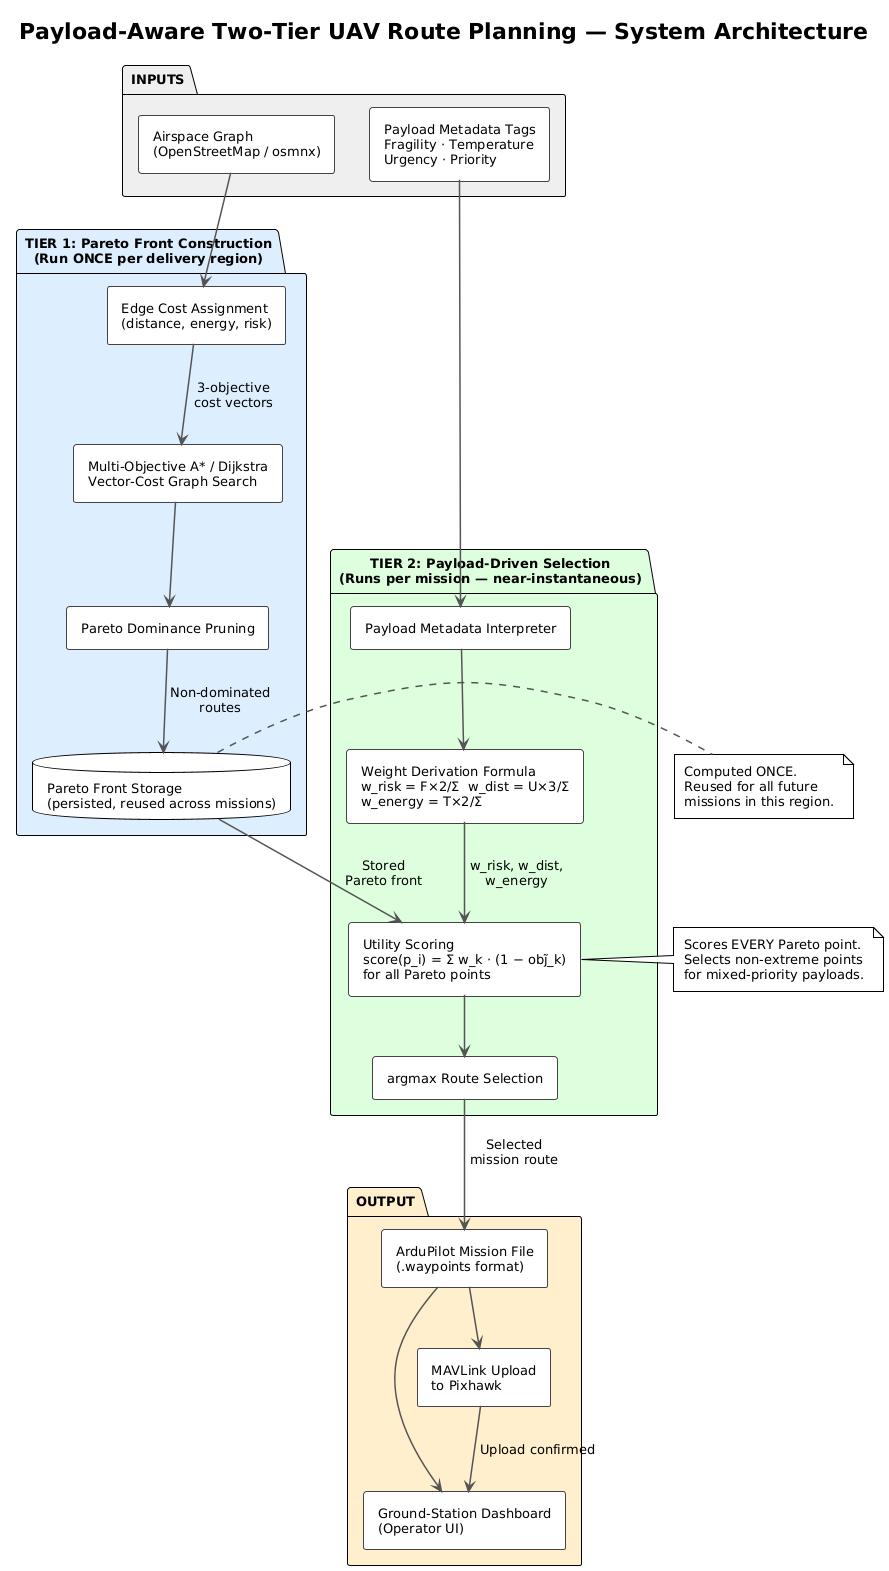
\includegraphics[width=0.78\textwidth]{arch.png}
\caption[Overall system architecture: Two-Tier Payload-Aware UAV Route Planner]{Overall
system architecture: Two-Tier Payload-Aware UAV Route Planner. Tier~1
pre-computes the Pareto front once per delivery region; Tier~2 selects the optimal route
for each new payload tag using the stored front.}\label{fig:architecture}
\end{figure}

The airspace graph $G = (V,E)$ is extracted from OpenStreetMap using the \texttt{osmnx}
Python library. Each edge $e \in E$ carries a cost vector:
\[
  \mathbf{c}(e) = \bigl[d(e),\; \varepsilon(e),\; \rho(e)\bigr]
\]
where $d(e)$ is the geodesic distance of the flight segment (km), $\varepsilon(e)$ is
the estimated energy consumption (proxy: $d(e) \times$ altitude-change factor), and
$\rho(e) \in [0,1]$ is the flight risk score derived from obstacle density, proximity to
no-fly zones, and wind exposure (simulated programmatically for reproducible
benchmarking).

The three optimisation objectives are: (1)~minimise route distance $d$; (2)~minimise
energy consumption $\varepsilon$; and (3)~minimise flight risk $\rho$. A route $p$
dominates route $q$ if $p$ is at least as good as $q$ on all three objectives and
strictly better on at least one. The Pareto front $\mathcal{P}$ is the set of all
non-dominated routes.

\textbf{Tier~2 Algebraic Bridge.} Each of the four payload metadata tags maps to exactly
one Tier~1 routing objective as shown in Table~\ref{tab:semantic-mapping}.

\begin{table}[H]
\centering\caption{Semantic mapping: payload metadata tags to Tier~1 routing objectives}\label{tab:semantic-mapping}\small
\begin{tabularx}{\textwidth}{L{2.8cm} L{1.4cm} Y L{4.2cm}}
\toprule
\textbf{Payload Tag} & \textbf{Range} & \textbf{Maps to Tier~1 Objective} & \textbf{Reasoning}\\
\midrule
Fragility class $F$      & 1--5 & $w_\mathrm{risk}$ (flight risk weight)   & Fragile items need low-vibration, low-risk corridors\\
Temperature sensitivity $T$ & 1--3 & $w_\mathrm{energy}$ (energy weight)  & Temp-sensitive items need short exposure time $\Rightarrow$ fast flight\\
Delivery urgency $U$     & 1--3 & $w_\mathrm{dist}$ (distance weight)       & Time-critical deliveries need the shortest path\\
Priority level $P_\mathrm{lvl}$ & 1--5 & Tie-breaker amplifier           & Scales the dominant weight when scores are close\\
\bottomrule
\end{tabularx}
\end{table}

From the payload tags, three routing objective weights are derived algorithmically with
no expert input:
\begin{align}
  r_\mathrm{raw} &= F \times 2, \quad d_\mathrm{raw} = U \times 3, \quad e_\mathrm{raw} = T \times 2 \label{eq:raw}\\
  w_\mathrm{risk} &= \frac{r_\mathrm{raw}}{r_\mathrm{raw} + d_\mathrm{raw} + e_\mathrm{raw}}, \quad
  w_\mathrm{dist} = \frac{d_\mathrm{raw}}{r_\mathrm{raw} + d_\mathrm{raw} + e_\mathrm{raw}}, \quad
  w_\mathrm{energy} = \frac{e_\mathrm{raw}}{r_\mathrm{raw} + d_\mathrm{raw} + e_\mathrm{raw}} \label{eq:weights}
\end{align}
The multipliers (2 for fragility and temperature, 3 for urgency) reflect the domain
insight that urgency has a higher penalty sensitivity than fragility or thermal
constraints in the UAV medical delivery context.

For each Pareto point $p_i$ with objective values $(d_i, \varepsilon_i, \rho_i)$,
min-max normalised values $\tilde{d}_i$, $\tilde{\varepsilon}_i$, $\tilde{\rho}_i$ are
computed over the full Pareto front $\mathcal{P}$. The utility score is:
\begin{equation}
  \mathrm{score}(p_i) = w_\mathrm{dist}\cdot(1 - \tilde{d}_i) + w_\mathrm{energy}\cdot(1 - \tilde{\varepsilon}_i) + w_\mathrm{risk}\cdot(1 - \tilde{\rho}_i) \label{eq:score}
\end{equation}
The selected mission route is $p^* = \arg\max_{p_i \in \mathcal{P}}\,\mathrm{score}(p_i)$.
For high-priority missions ($P_\mathrm{lvl} \geq 4$), the dominant weight is amplified
by $0.1 \times w_\mathrm{max}$ to sharpen the selection.

The Tier~1 and Tier~2 activity flows are shown in Figures~\ref{fig:tier1} and
\ref{fig:tier2} respectively.

\begin{figure}[H]
\centering
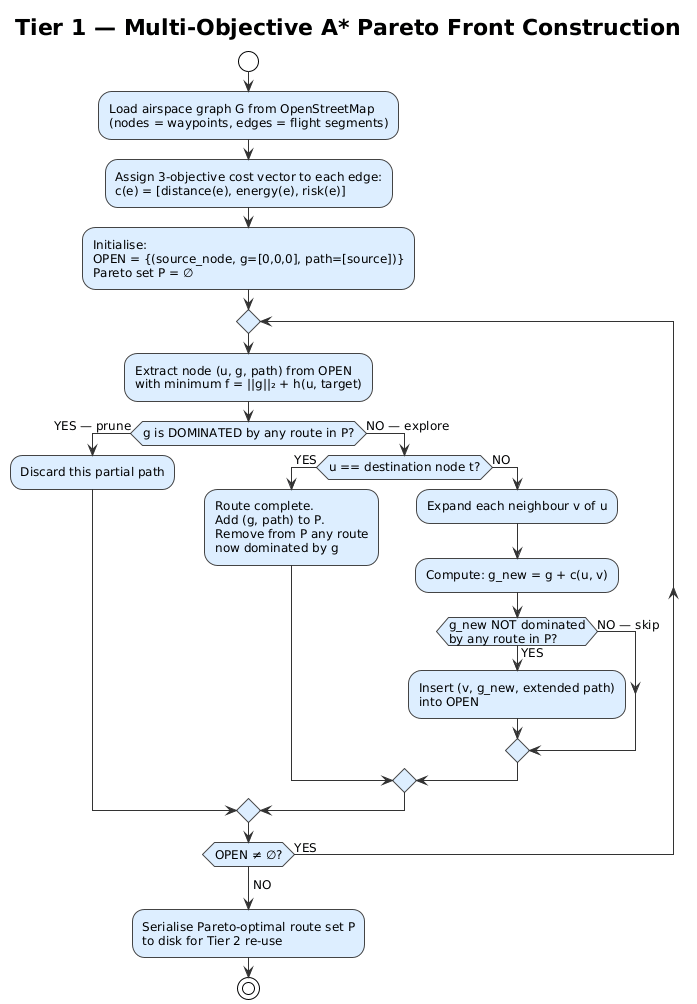
\includegraphics[width=0.82\textwidth]{tier1.png}
\caption[Tier~1 activity flow: Multi-Objective A* Pareto Front Construction]{Tier~1
activity flow: Multi-Objective A* Pareto Front Construction. The open
set is explored in order of estimated total cost until no further non-dominated routes
exist.}\label{fig:tier1}
\end{figure}

\begin{figure}[H]
\centering
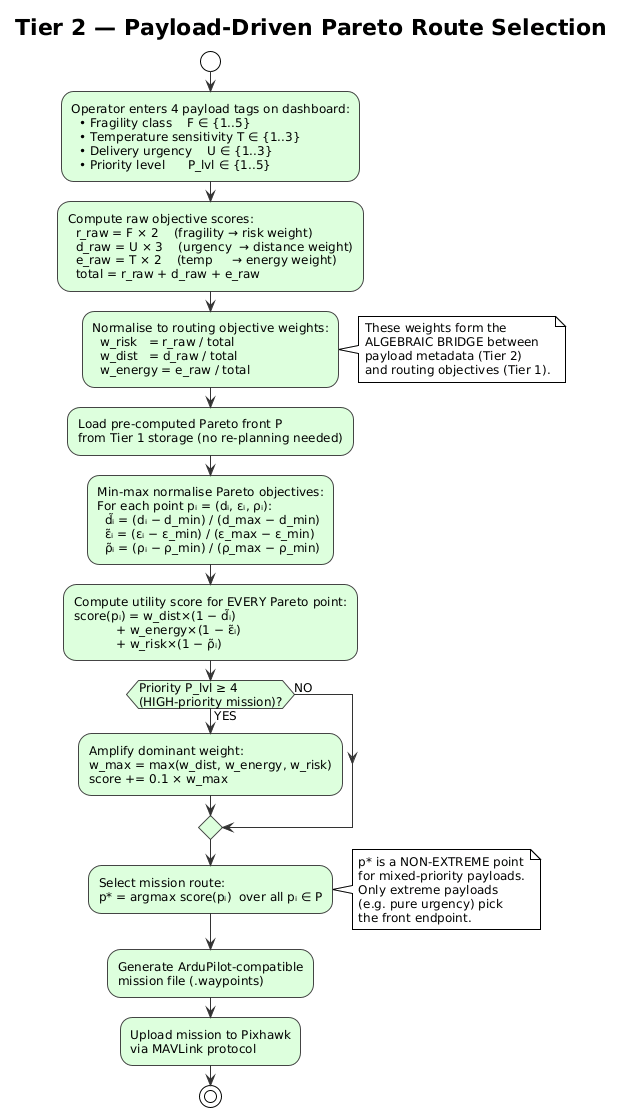
\includegraphics[width=0.82\textwidth]{tier2.png}
\caption[Tier~2 activity flow: Payload-Driven Pareto Selection]{Tier~2 activity flow:
Payload-Driven Pareto Selection. Payload tags are
algebraically mapped to weights, which score every Pareto point via a utility function;
the $\arg\max$ is selected as the mission route.}\label{fig:tier2}
\end{figure}

\section{Modules}

\subsection{Module 1: Airspace Graph Builder}
Extracts the road/path network from OpenStreetMap for a specified delivery region using
\texttt{osmnx}. Assigns three objective costs to each edge: geodesic distance, energy
(distance $\times$ altitude-change factor), and flight risk (simulated threat zones and
obstacle density scored 0--1 using a configurable hazard map). Output: a directed
weighted graph $G$ stored as a serialised NetworkX object ready for Tier~1 search.

\subsection{Module 2: Multi-Objective A*/Dijkstra Engine (Tier~1)}
Implements the multi-objective A* algorithm maintaining a cost vector $\mathbf{g}$ (not
a scalar) for each partial path. Paths dominated by already-discovered routes are pruned
early. The \texttt{UpdateParetoFront} subroutine adds a new route and removes any
previously stored routes it dominates. Output: a deterministic, reproducible Pareto
front $\mathcal{P}$ serialised to disk for Tier~2 re-use across all future missions in
the same delivery region.

\subsection{Module 3: Payload Metadata Interpreter (Tier~2)}
Implements the payload-driven route selection algorithm: reads the four payload tags,
derives objective weights via Equations~(\ref{eq:raw})--(\ref{eq:weights}), applies
min-max normalisation to Pareto objectives, computes a utility score for every Pareto
point via Equation~(\ref{eq:score}), and returns the $\arg\max$ route. Optionally
amplifies the dominant weight for high-priority missions ($P_\mathrm{lvl} \geq 4$).
Generates an ArduPilot-compatible \texttt{.waypoints} mission file for upload.

\subsection{Module 4: Testing and Evaluation}
Evaluates all methods on three scenario scales: S1 (${\approx}50$ nodes, low obstacle
density), S2 (${\approx}200$ nodes, medium density), and S3 (${\approx}500$ nodes, high
density). The MOPSO baseline runs with swarm size 100, 200 iterations, and a Pareto
archive of 100 solutions, repeated 30 times per scenario to obtain mean $\pm$ standard
deviation. Metrics include Hypervolume (HV), Inverted Generational Distance (IGD), and
Tier~2 selection accuracy across four payload presets. Phase~II testing extends to
ArduPilot SITL validation and outdoor flight tests on an F450 quadcopter with Pixhawk
flight controller, measuring route adherence (GPS position error vs.\ planned route) and
end-to-end latency.

% ============================================================
\chapter{Project Timeline Chart}\label{cha:timeline}

\begin{figure}[H]
\centering
\resizebox{\textwidth}{!}{%
\begin{ganttchart}[
  hgrid,
  vgrid,
  time slot format=isodate-yearmonth,
  time slot unit=month,
  title label font=\bfseries\footnotesize,
  bar label font=\small,
  bar label node/.append style={align=left, text width=4.8cm},
  bar/.append style={fill=blue!45},
  milestone/.append style={fill=red!80},
  x unit=1.55cm,
  y unit title=0.60cm,
  y unit chart=0.52cm
]{2026-07}{2027-03}
\gantttitlecalendar{year, month=shortname}\\
\ganttbar{Literature Survey \& Problem Formulation}{2026-07}{2026-09}\\
\ganttbar{System Design \& Architecture}{2026-09}{2026-10}\\
\ganttmilestone{Review I}{2026-08}\\
\ganttbar{Tier 1: Multi-Objective A* Engine}{2026-10}{2026-11}\\
\ganttbar{Tier 2: Payload-Driven Selector}{2026-11}{2026-12}\\
\ganttbar{Software Simulation \& Benchmarking}{2026-12}{2027-01}\\
\ganttbar{Hardware Integration (RPi 5 + Pixhawk)}{2027-01}{2027-02}\\
\ganttbar{Outdoor Flight Tests \& Evaluation}{2027-02}{2027-03}\\
\ganttbar{Documentation \& Report Writing}{2027-02}{2027-03}\\
\ganttmilestone{Final Submission}{2027-03}
\end{ganttchart}}
\caption{Project timeline (July 2026 -- March 2027). Red diamonds mark review and
submission milestones.}\label{fig:timeline}
\end{figure}

% ============================================================
\begin{thebibliography}{99}

\bibitem{r1} B. Chokkalingam and S. Ganesan, ``Multi-objective UAV path planning with
adaptive constraint handling and entropy-based Pareto selection,''
\textit{RAIRO -- Operations Research}, 2026.

\bibitem{r2} O. Datsko et al., ``Diversity-driven Pareto selection for UAV routing,''
\textit{IEEE Robotics and Automation Letters (RA-L)}, vol.~9, 2024.

\bibitem{r3} C. Ntakolia et al., ``Crowding-distance Pareto selection in a multi-objective
UAV path planner,'' \textit{Journal of Intelligent \& Robotic Systems}, vol.~107, 2023.

\bibitem{r4} G. Boeing, ``OSMnx: New methods for acquiring, constructing, analysing, and
visualising complex street networks,'' \textit{Computers, Environment and Urban Systems},
vol.~65, pp.~126--139, 2017. DOI: \url{https://doi.org/10.1016/j.compenvurbsys.2017.05.004}.

\bibitem{r5} A. Hagberg, P. Swart, and D. Chult, ``Exploring network structure,
dynamics, and function using NetworkX,'' in \textit{Proc.\ 7th Python in Science Conf.\
(SciPy)}, pp.~11--15, 2008.

\bibitem{r6} C. A. C. Coello, G. T. Pulido, and M. S. Lechuga, ``Handling multiple
objectives with particle swarm optimization,'' \textit{IEEE Trans.\ Evolutionary
Computation}, vol.~8, no.~3, pp.~256--279, 2004.
DOI: \url{https://doi.org/10.1109/TEVC.2004.826067}.

\bibitem{r7} L. Meier et al., ``MAVLink: Micro air vehicle communication protocol,''
2013. [Online]. Available: \url{https://mavlink.io}. [Accessed: 24-Aug-2026].

\end{thebibliography}

\end{document}
